\section{Monte Carlo method}

\begin{wideslide}{Buffon's needle problem}
\null\vfill

  \twocolumn
  {
    {\it Suppose we have a floor made of parallel strips of wood, each the same width, and we drop a needle onto the floor. What is the probability that the needle will lie across a line between two strips?}
    
    \sep
    
    {\it\hfill Georges-Louis Leclerc,\\\hfill Comte de Buffon\\\hfill 18th century}
  }
  {
    \sep\sep
    \centering\begin{tikzpicture}[node distance = 0cm]
 
  \node (a) [rectH, filled2=pdcolor1, line width = 0] {};
  \node (b) [rectH, notFilled=pdcolor1, line width = 0, right=of a] {};
  \node (c) [rectH, filled2=pdcolor1, line width = 0, right=of b] {};
  \node (d) [rectH, notFilled=pdcolor1, line width = 0, right=of c] {};
  \node (e) [rectH, filled2=pdcolor1, line width = 0, right=of d] {};
  \node (f) [rectH, notFilled=pdcolor1, line width = 0, right=of e] {};
  
  \draw[color = pdcolor7, ultra thick, xshift=0.1cm, yshift=0.0cm, rotate=45] (0,0) -- (0.4,0);
  \draw[color = pdcolor6, ultra thick, xshift=1.4cm, yshift=-0.8cm, rotate=35] (0,0) -- (0.4,0);
  \draw[color = pdcolor7, ultra thick, xshift=2.0cm, yshift=-0.4cm, rotate=-30] (0,0) -- (0.4,0);
  \draw[color = pdcolor6, ultra thick, xshift=2.5cm, yshift=0.6cm, rotate=60] (0,0) -- (0.4,0);
  \draw[color = pdcolor6, ultra thick, xshift=0.8cm, yshift=-0.5cm, rotate=-20] (0,0) -- (0.4,0);
  \draw[color = pdcolor7, ultra thick, xshift=1.1cm, yshift=0.3cm, rotate=15] (0,0) -- (0.4,0);
 
  \node(red) [below=of c, yshift=-0.1cm] {\color{pdcolor7} blue are good};
  \node(blue) [below=of red] {\color{pdcolor6} red are bad};
 
\end{tikzpicture}

  }
  
  \vspace{-10pt}
  \myBoxFullWidth{Monte Carlo without computers}
  
  \twocolumn
  {
    If needle length ($l$) $<$ lines width ($t$):
    
    $$P = \frac{2l}{t\pi}$$
    
    which can be used to estimate $\pi$:
    
    $$\pi = \frac{2l}{tP}$$
  }
  {
    MC experiment was performed by Mario Lazzarini in 1901 by throwing 3408 needles:
    
    $$\pi = \frac{2l \cdot 3408}{t \cdot \#red} = \frac{355}{113} = 3.14159292$$
  }
  
\vfill\null
\end{wideslide}

\begin{wideslide}[toc = From Solitaire to MC]{From Solitaire to Monte Carlo method}
\null\vfill

    \twocolumn
    {
      \begin{itemize}
	\item Stanis{\l}aw Ulam was a Polish mathematician
	\item He invented the Monte Carlo method while playing solitaire
	\item The method was used in Los Alamos, performed by ENIAC computer
      \end{itemize}  
      
      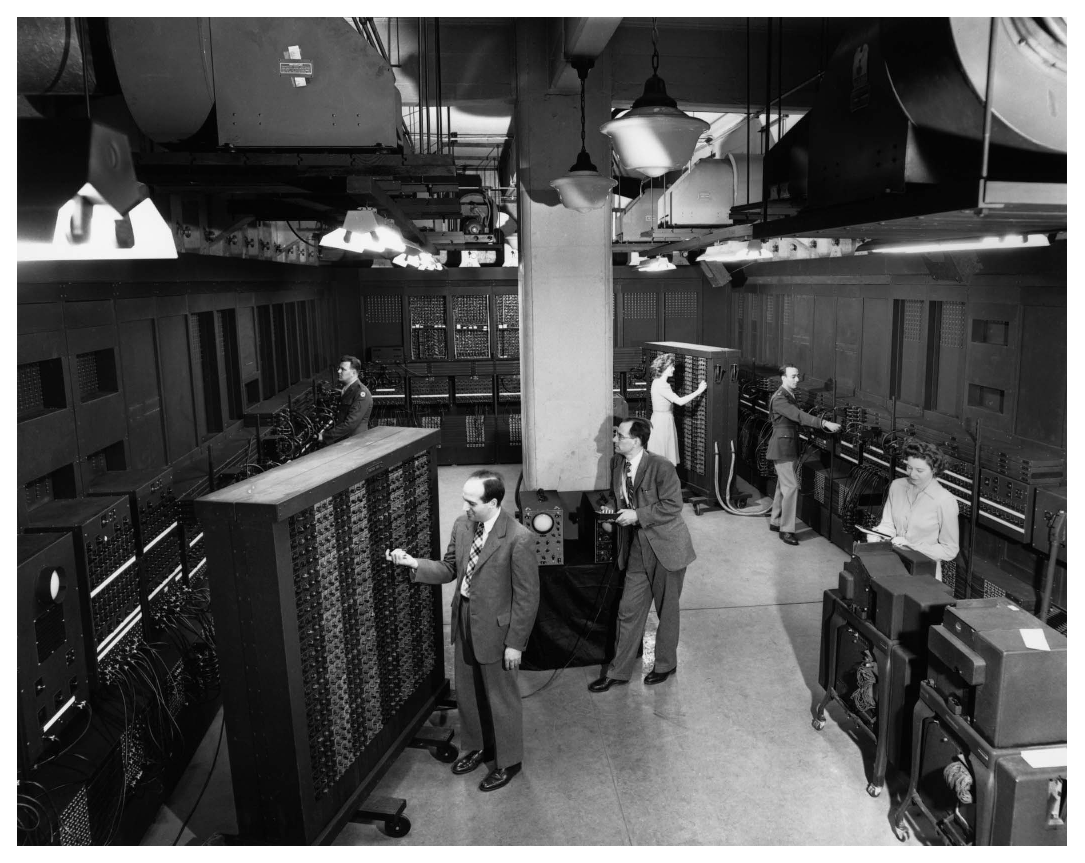
\includegraphics[width=\columnwidth]{figures/eniac1946.eps}
    }
    {
      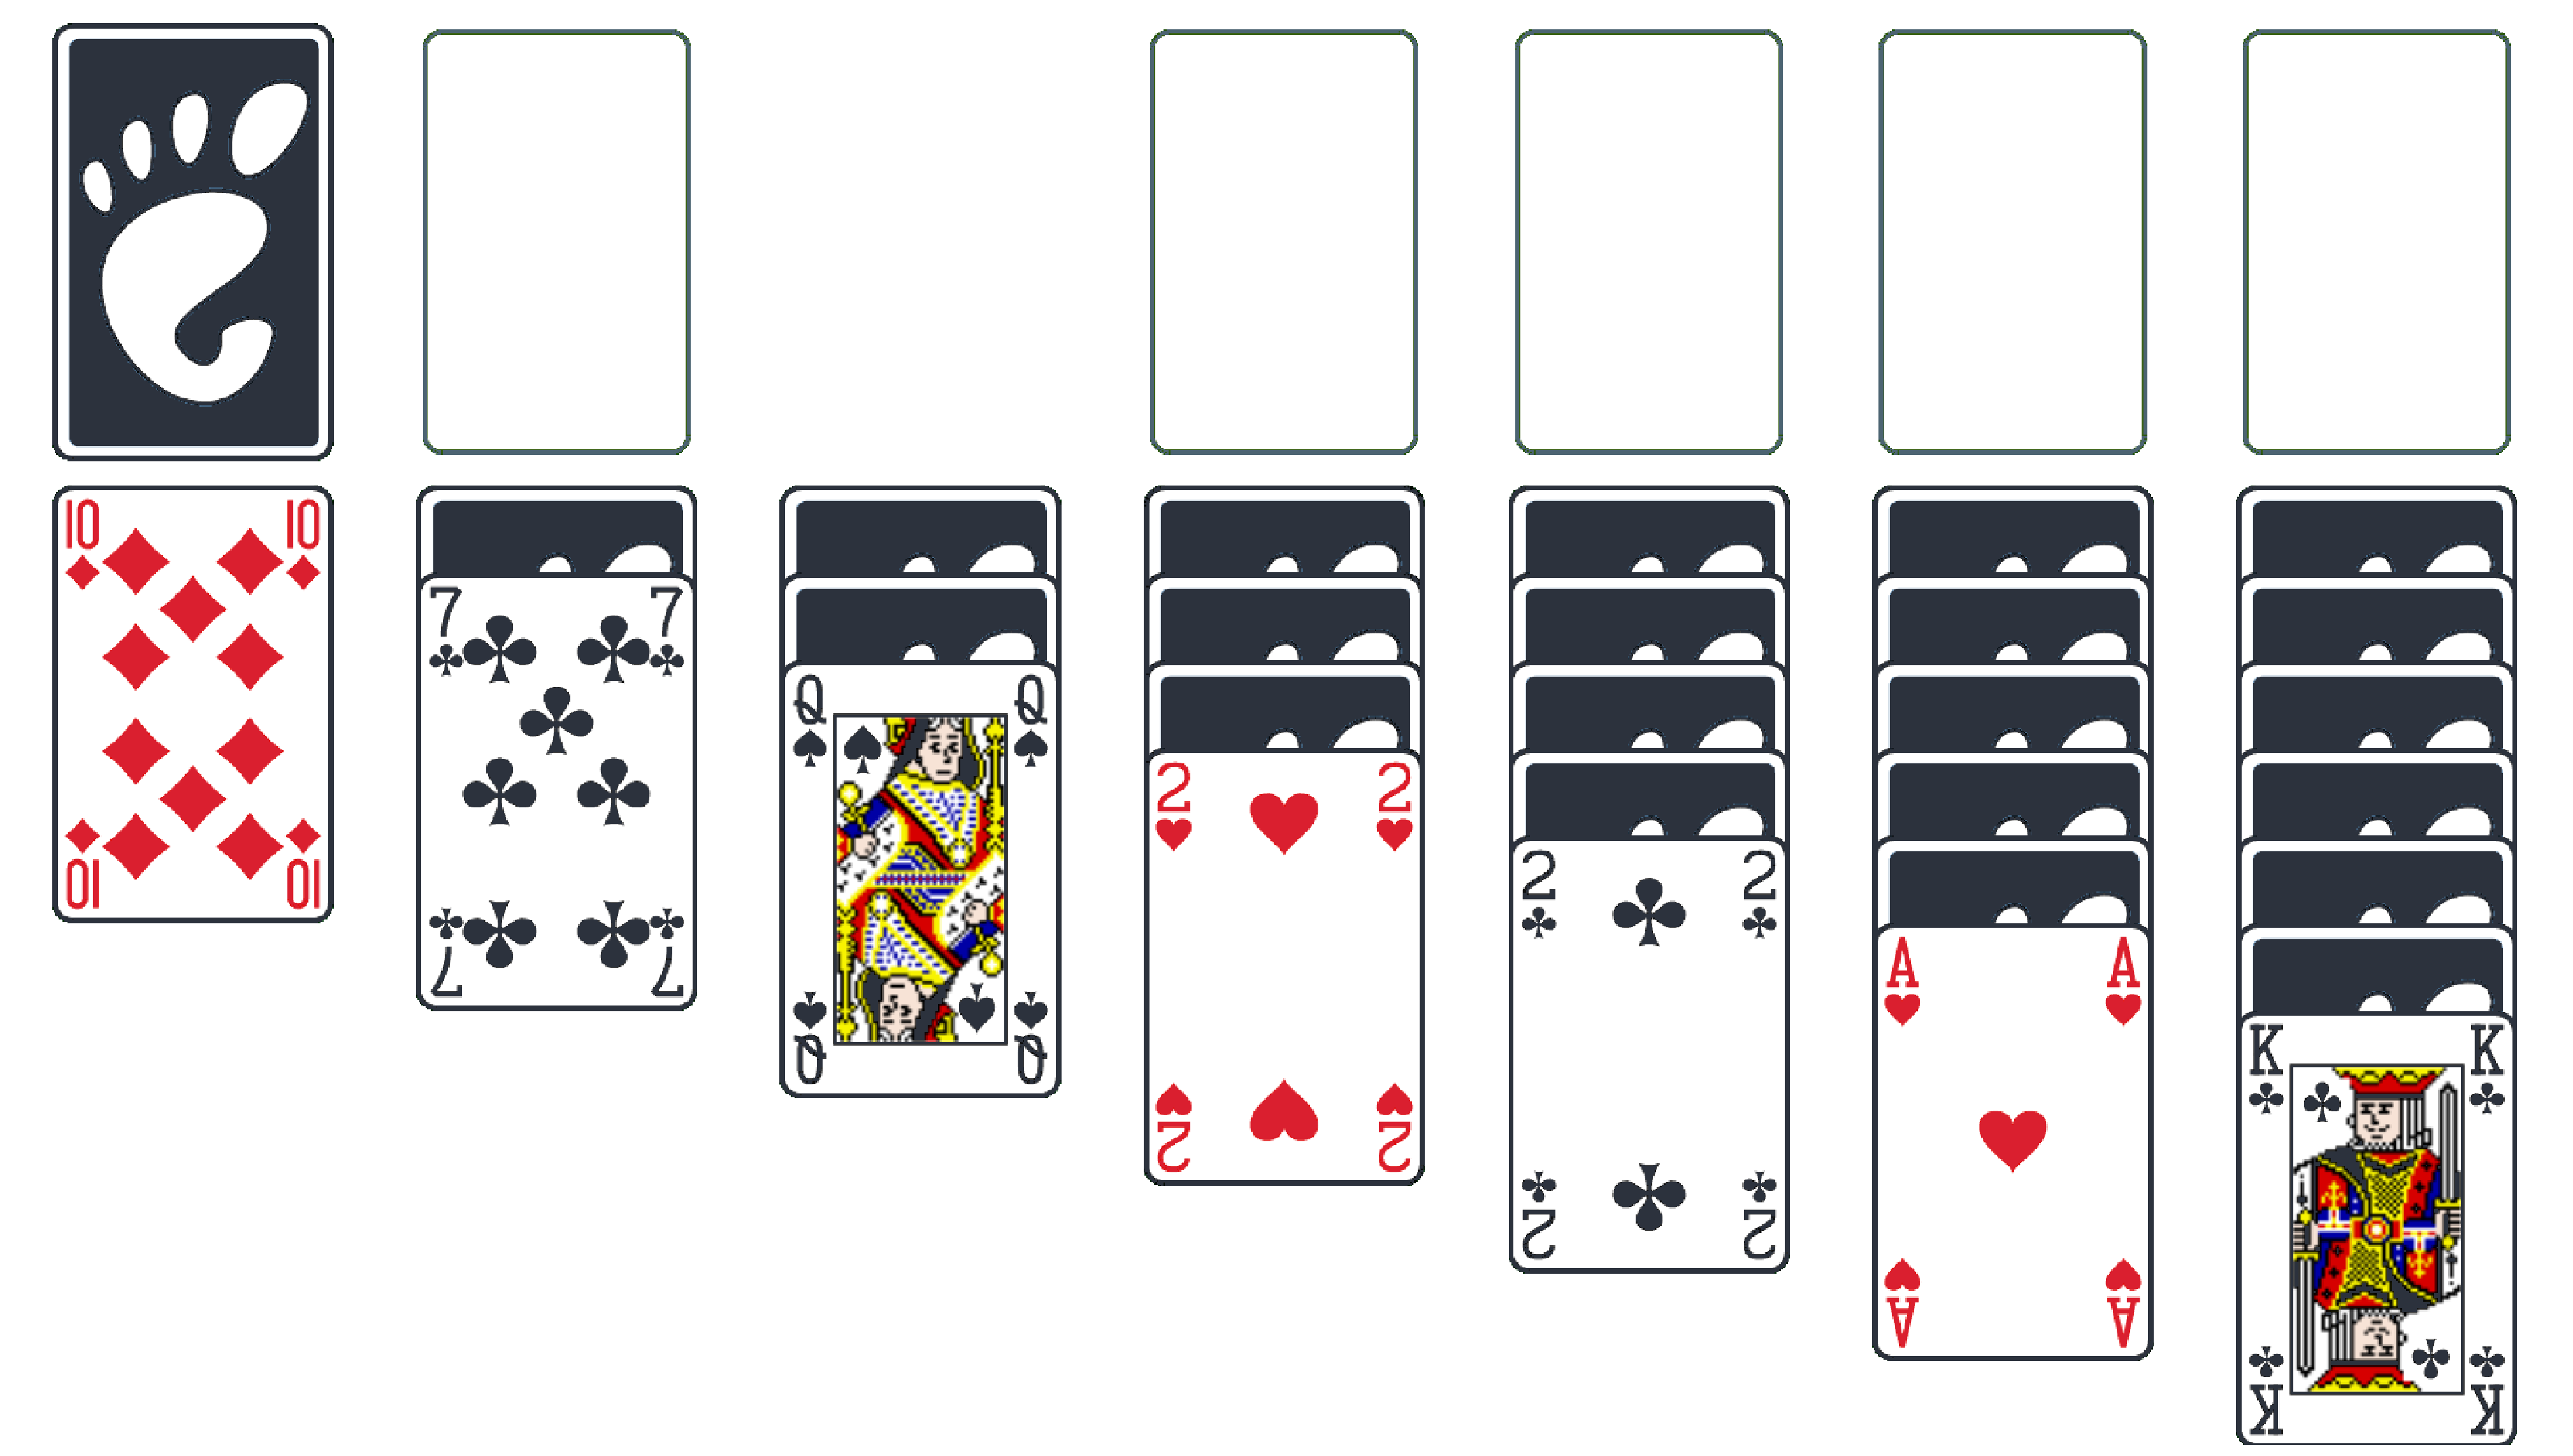
\includegraphics[width=\columnwidth]{figures/solitaire.eps}
      \begin{itemize}
	\item What is a probability of success in solitaire?
	\begin{itemize}
	  \item Too complex for an analytical calculations
	  \item Lets try $N = 100$ times and count wins
	  \item With $N \rightarrow \infty$ we are getting closer to correct result
	\end{itemize}
      \end{itemize}
    }
 
\vfill\null
\end{wideslide}

\begin{wideslide}[toc = Simple Monte Carlo, method=direct]{Simple Monte Carlo - coin flipping}
\null\vfill

  \begin{itemize}
    \item What is the probability of getting head / tail when throwing a coin?
  \end{itemize}
  
  \begin{minipage}{0.7\textwidth}
  \begin{itemize}
    \item One can use MC method to calculate this:
    \begin{itemize}
      \item get $N$ times a random number $x \in [0,1)$
      \item check how many ($n$) times $x < 0.5$
      \item $P = \frac{n}{N}$
    \end{itemize}
    \item One-line example in Python:
  \end{itemize}
  \end{minipage}\begin{minipage}{0.3\textwidth}
		  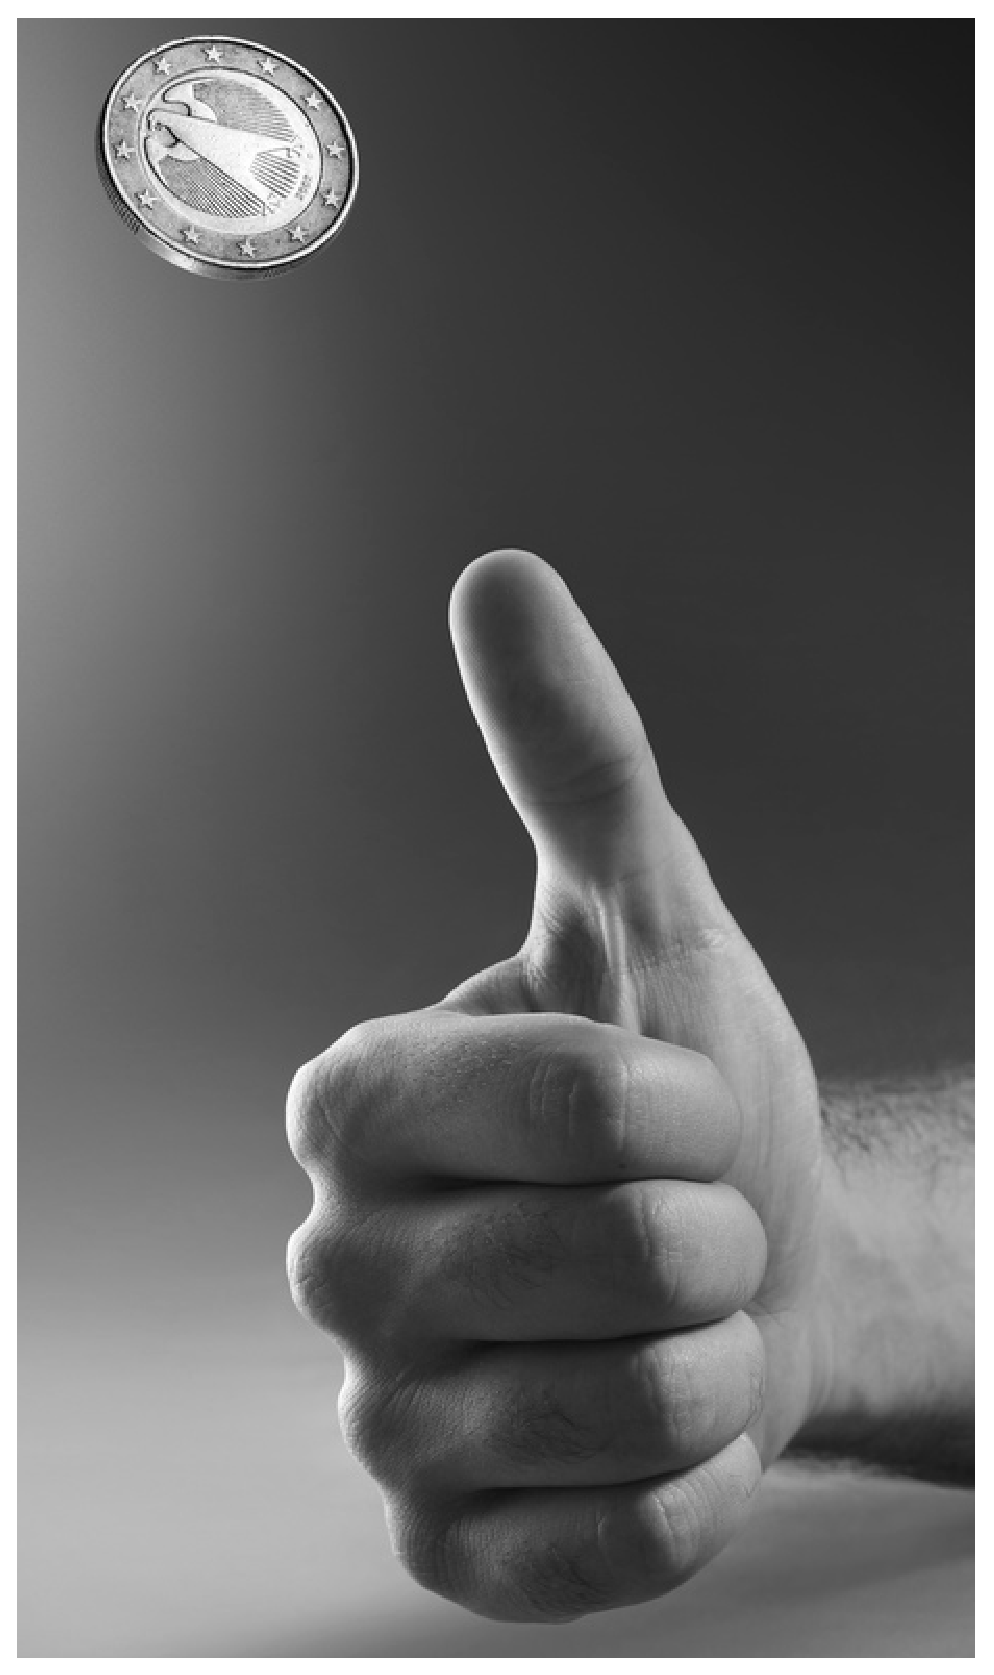
\includegraphics[width=0.5\columnwidth]{figures/coin.eps}
                \end{minipage}

  {\small\color{pdcolor3}
  \begin{verbatim}
MC = lambda N: len(filter(lambda x: random.random() < 0.5, range(N))) / float(N)     
  \end{verbatim}
  }
  \begin{minipage}{0.55\textwidth}
  \begin{itemize}
   \item If you do not like one-liners:
  \end{itemize}
  \vspace{-20pt}  
  {\small\color{pdcolor3}
  \begin{verbatim}
def MonteCarlo(N):
  n = 0
  for _ in range(N):
    if (random.random() < 0.5): n += 1
  return float(n) / N   
  \end{verbatim}
  }
  \end{minipage}\begin{minipage}{0.45\textwidth}
		  \vspace{-10pt}
		  \begin{itemize}
		   \item Some results for MC(100):
		   \item[]
		   0.51, 0.48, 0.61, 0.46, 0.57, 0.46
		   \item Some results for MC(100000):
		   \item[]
		   0.50139, 0.49798, 0.49933, 0.5005
		  \end{itemize}
                \end{minipage}

\vfill\null
\end{wideslide}

\begin{slide}[toc=PRNG]{Pseudorandom number generator}
\null\vfill

  \begin{itemize}
    \item PRNG is an algorithm for generating a sequence of ``random'' numbers
    \item Example: middle-square method (used in ENIAC)
    \begin{itemize}
      \item take $n$-digit number as your seed
      \item square it to get $2n$-digit number (add leading zeroes if necessary)
      \item $n$ middle digits are the result and the seed for next number
    \end{itemize}
    \item Middle-square method for $n = 4$ and base seed = $1111$:
  \end{itemize}
  \vspace{-10pt}
  \begin{eqnarray*}
    1111^2 & = & {\color{pdcolor3}01}2343{\color{pdcolor3}21} \rightarrow 2343 \\
    2343^2 & = & {\color{pdcolor3}05}4896{\color{pdcolor3}49} \rightarrow 4896 \\
    & \vdots & \\
    1111^2 & = & {\color{pdcolor3}01}2343{\color{pdcolor3}21} \rightarrow 2343 
  \end{eqnarray*}
    
\vfill\null
\end{slide}

\begin{slide}[toc=]{Pseudorandom number generator}
\null\vfill

  \begin{itemize}
    \item Nowadays, more sophisticated PRNGs exist, but they also suffer on some common problems:
    \begin{itemize}
      \item periodicity / different periodicity for different base seed
      \item nonuniformity of number distributions
      \item correlation of successive numbers
    \end{itemize}
  \end{itemize}

  \twocolumn
  {
    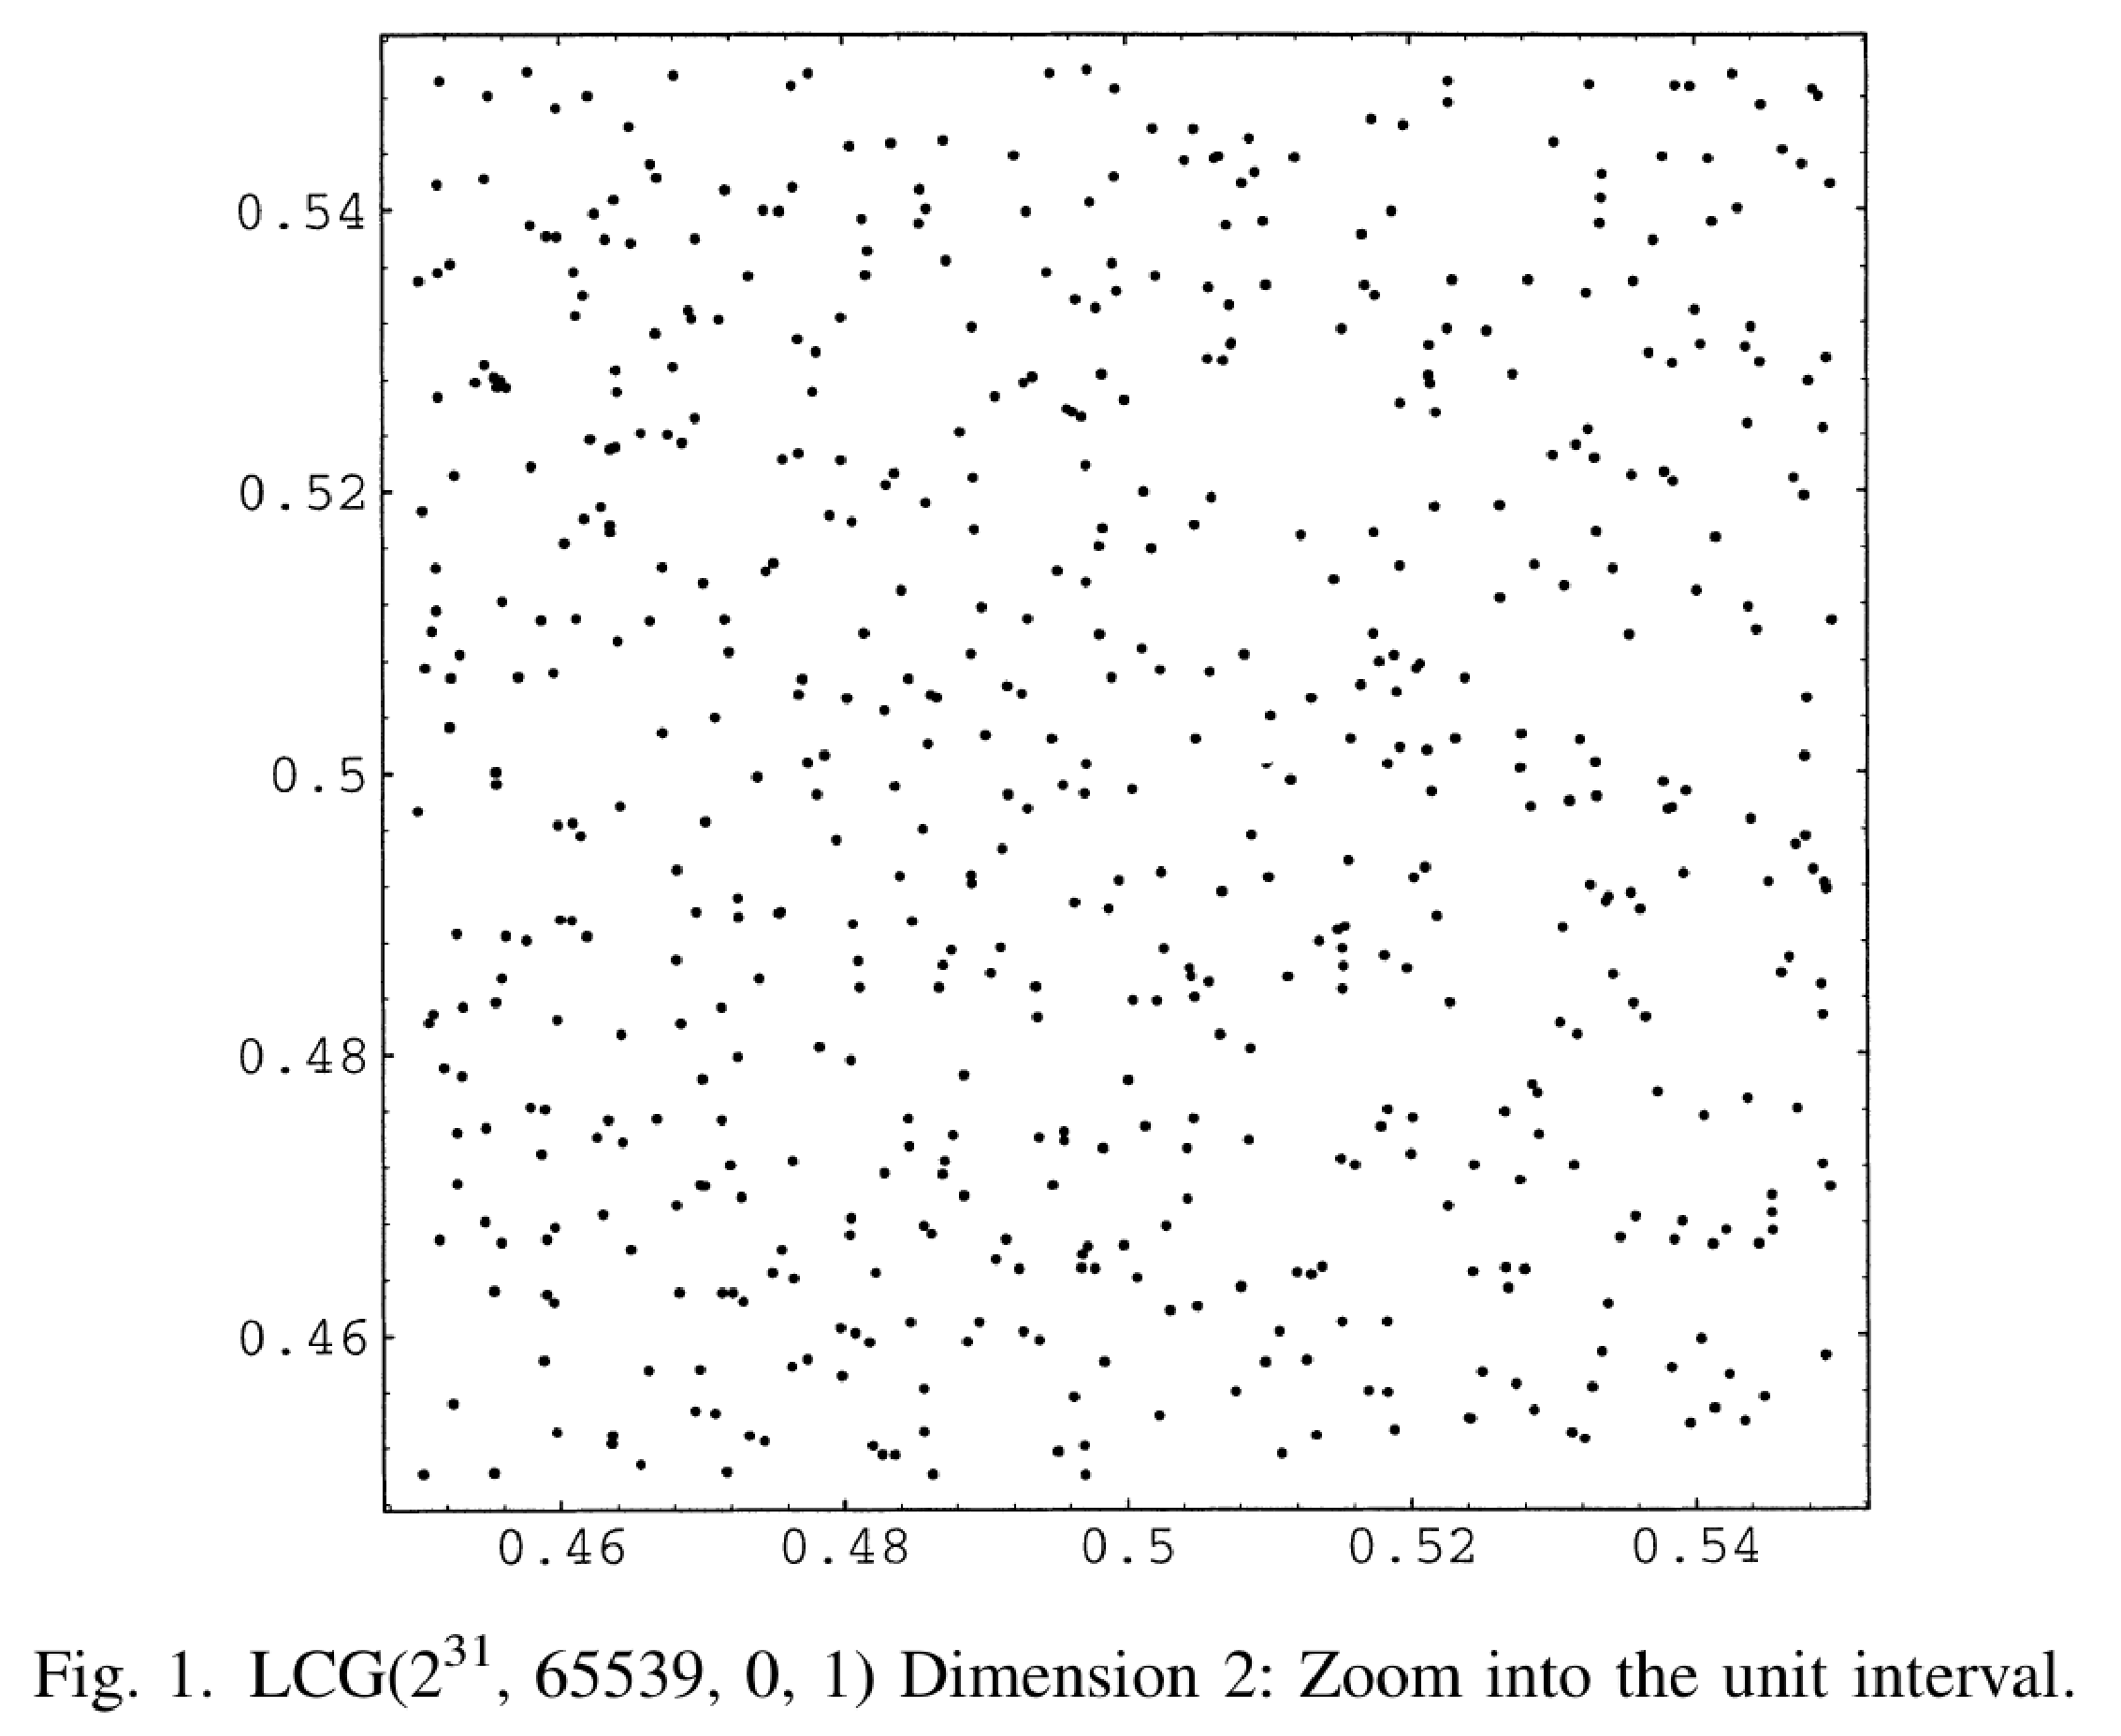
\includegraphics[width=\columnwidth]{figures/random2d.eps}
  }
  {
    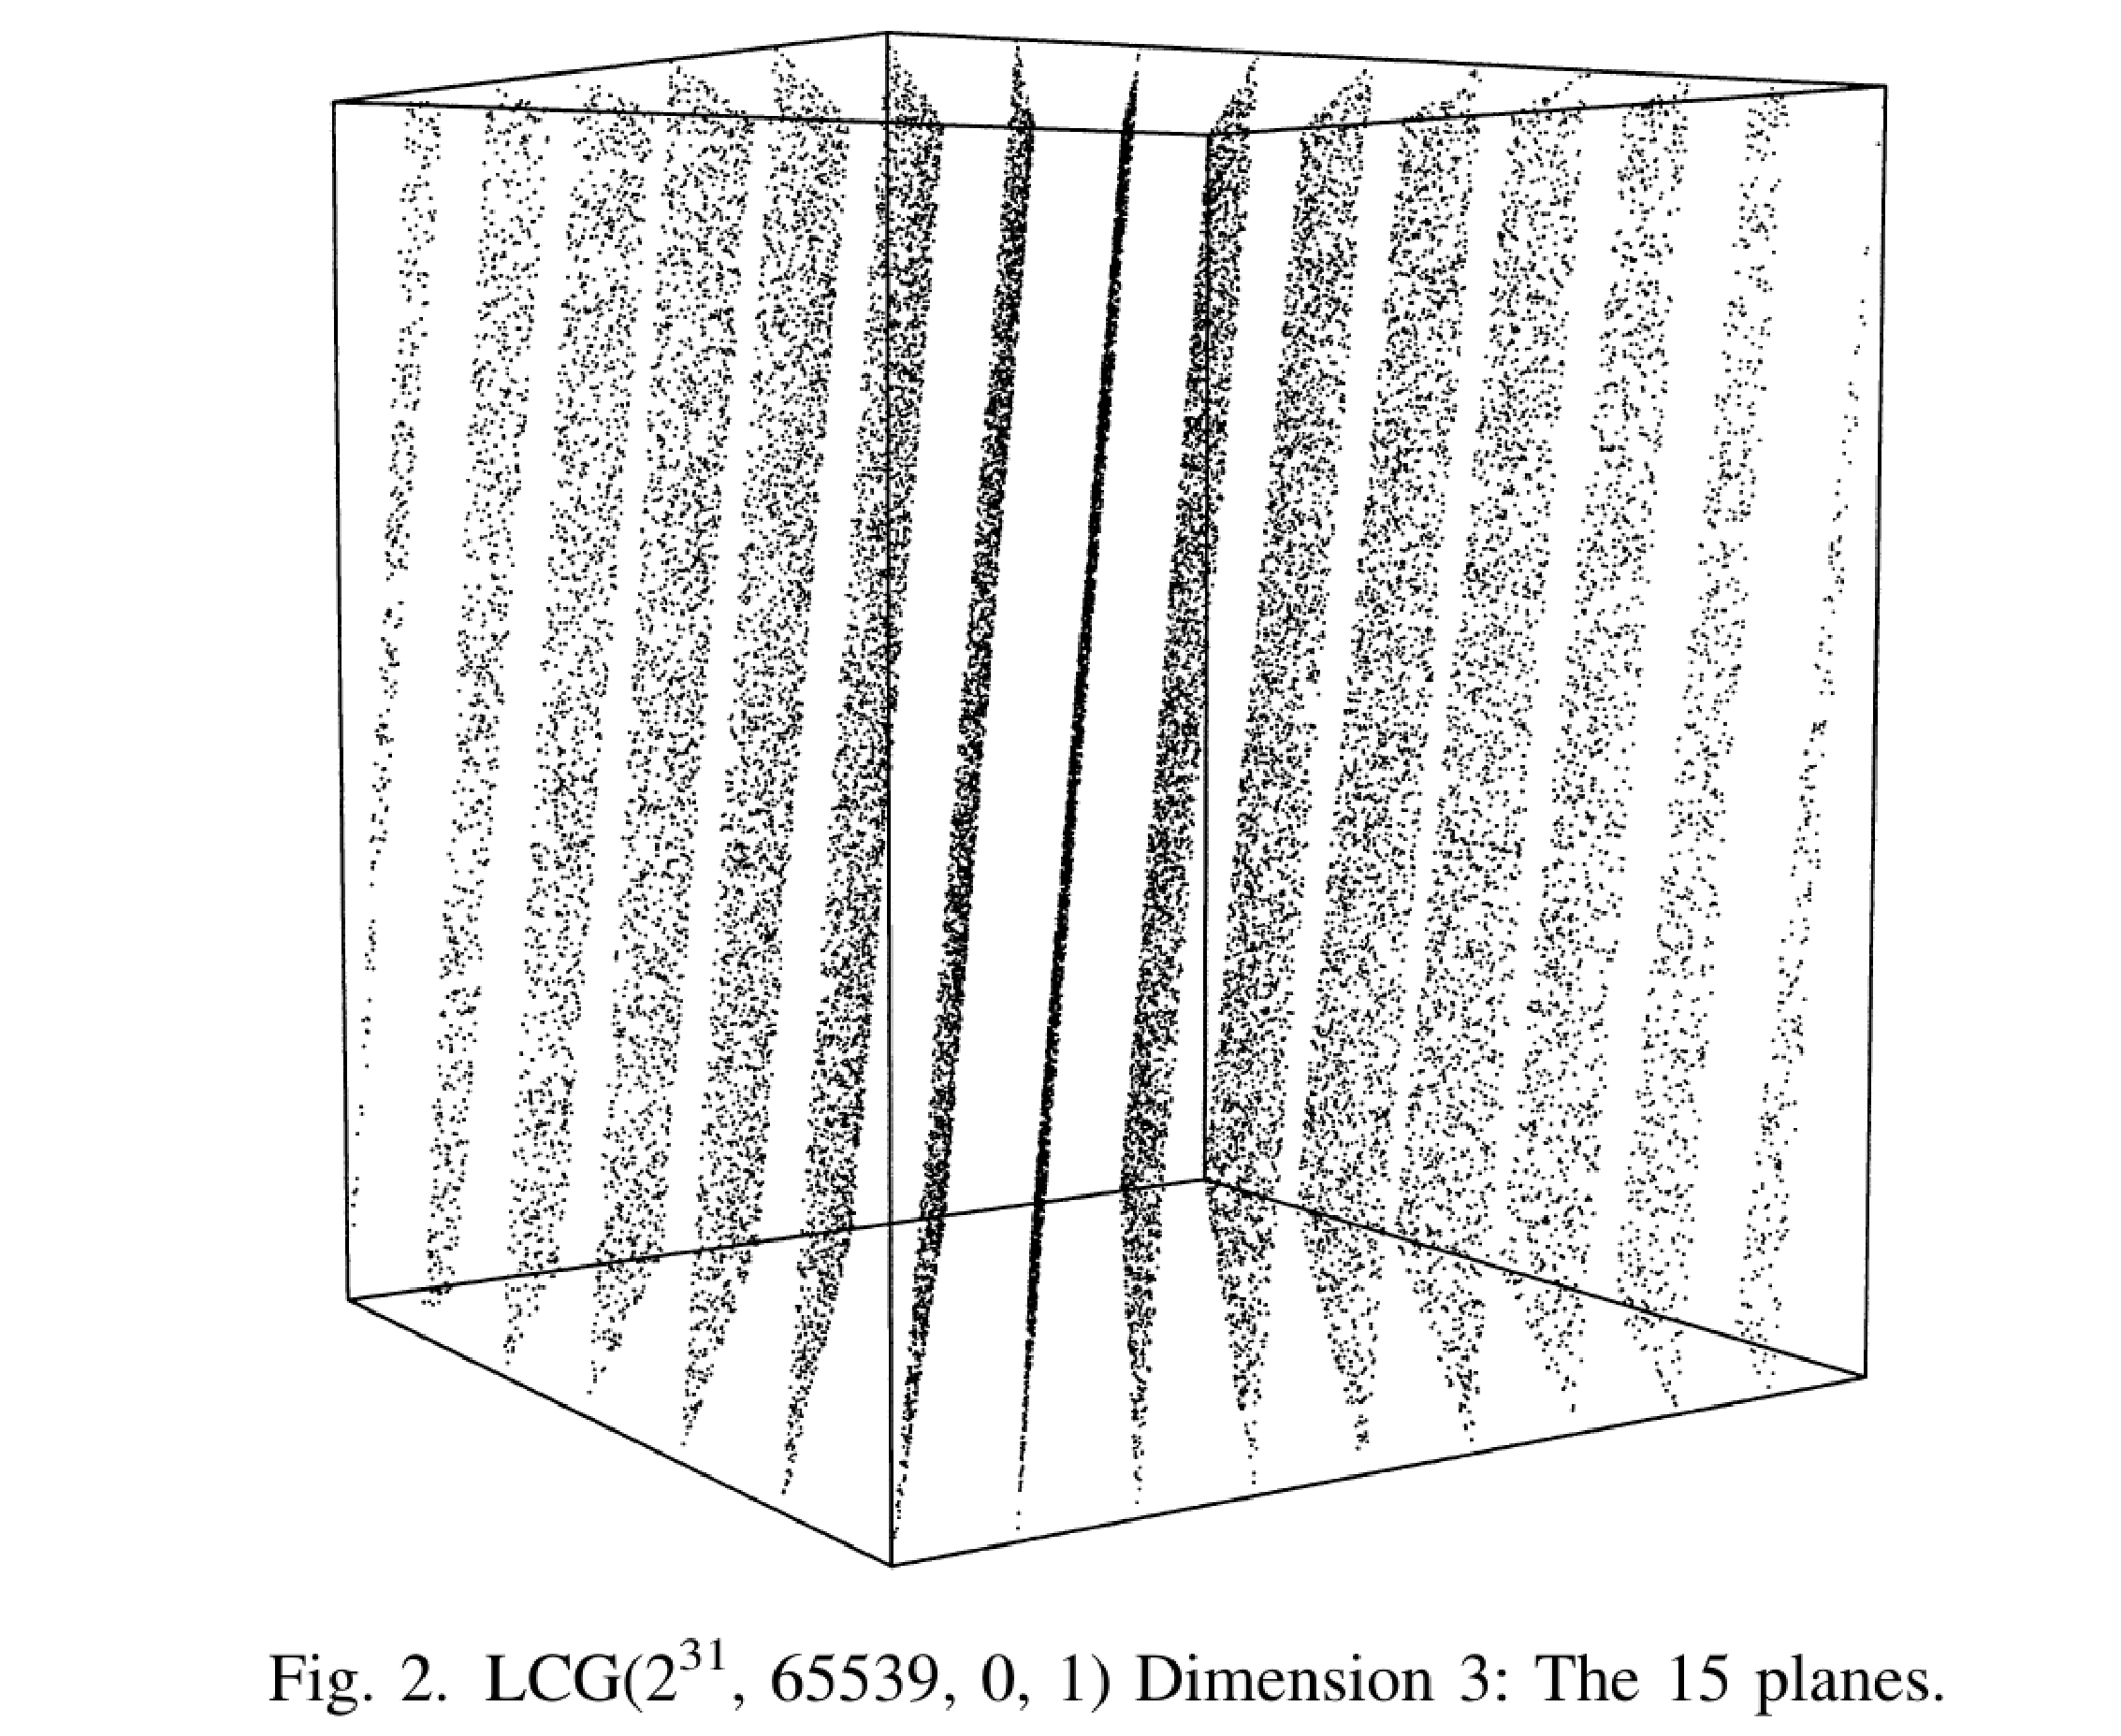
\includegraphics[width=\columnwidth]{figures/random3d.eps}
  }
  {\it\color{pdcolor3}Mathematics and Computers in Simulations 46 (1998) 485-505}
\vfill\null
\end{slide}

\begin{slide}[toc=Hit-or-Miss method]{MC integration (Hit-or-Miss method)}
\null\vfill

  Lets do the following integration using MC method:
  
  $$\int_0^1 f(x)dx = \int_0^1 \left(\frac{1}{2}x\right) dx = \left.\frac{1}{2}\frac{x^2}{2}\right|_{0}^{1} = \frac{1}{4}$$

  \twocolumn
  {
    \sep
    \begin{itemize}
     \item take a random point from the $[0,1]\times[0,1]$ square
     \item compare it to your $f(x)$
     \item repeat $N$ times
     \item count $n$ points below the function
     \item you results is given by
     $$\int_0^1 f(x)dx = P_{\square} \cdot \frac{n}{N} = \frac{n}{N}$$
    \end{itemize}
  }
  {
    \usetikzlibrary{calc}

\begin{tikzpicture}

  \draw[>=latex, <->, thick] node[left, yshift = 4cm]{$y$} ++ (0, 4) -- (0, 0) -- node[below, xshift = 2cm]{$x$} ++ (4,0);
  
  \foreach \x in {1,...,200}
  {
    \pgfmathparse{rnd}
    \pgfmathsetmacro{\a}{2.9*\pgfmathresult + 0.05}
    \pgfmathparse{rnd}
    \pgfmathsetmacro{\b}{2.9*\pgfmathresult + 0.05}
    \pgfmathsetmacro{\c}{\a - 2.0 * \b}
        
    \ifthenelse{\lengthtest{\c pt > 0.2 pt}}{\draw[filled, color=pdcolor7] (\a, \b) circle (0.03);}{}
    \ifthenelse{\lengthtest{\c pt < - 0.2 pt}}{\draw[filled, color=pdcolor6] (\a, \b) circle (0.03);}{}
  }

  \draw[ultra thick] (0,0) -- node[yshift = 1.5cm, xshift = 2cm]{$f(x) = \frac{1}{2}x$} ++ (4,2);
  
  \draw[color=pdcolor3, dashed] node[left, yshift = 3cm]{1} ++ (0, 3) -- (3,3) -- node[yshift = -1.75cm]{1} (3, 0);
      
\end{tikzpicture}

  }
  
\vfill\null
\end{slide}

\begin{emptyslide}{MC integration results}
\null\vfill

  \twocolumn
  {
    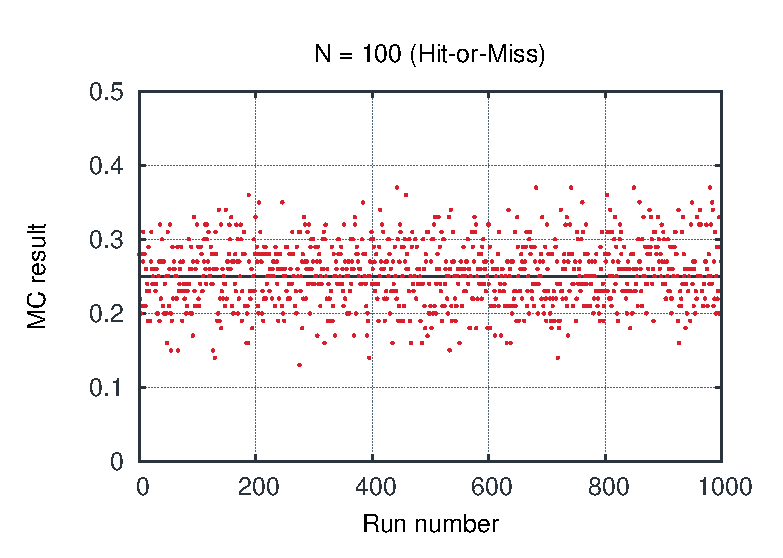
\includegraphics[width=\columnwidth]{figures/int100.eps}
    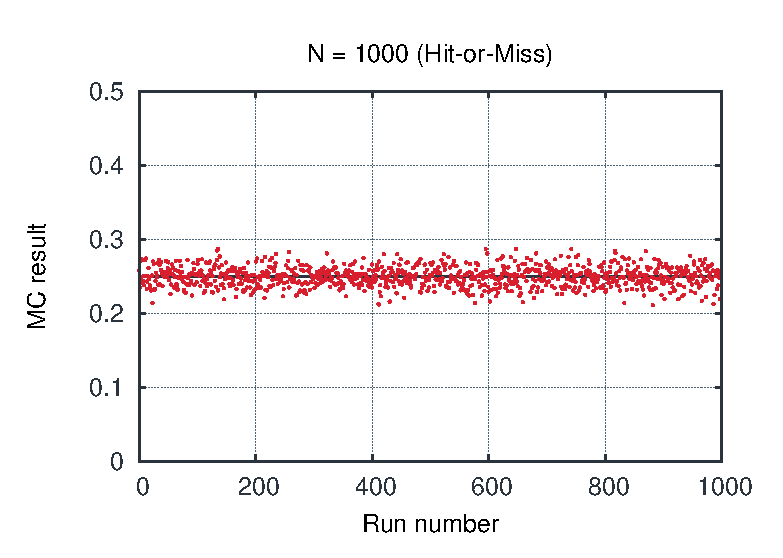
\includegraphics[width=\columnwidth]{figures/int1000.eps}
  }
  {
    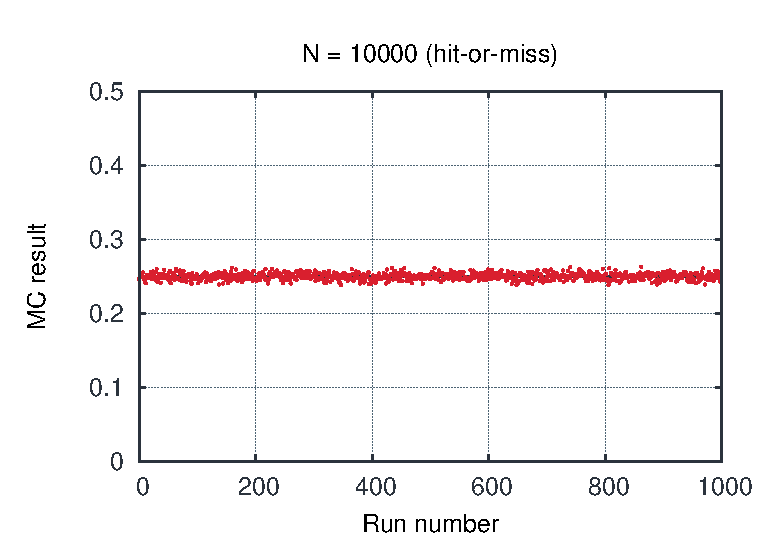
\includegraphics[width=\columnwidth]{figures/int10000.eps}
    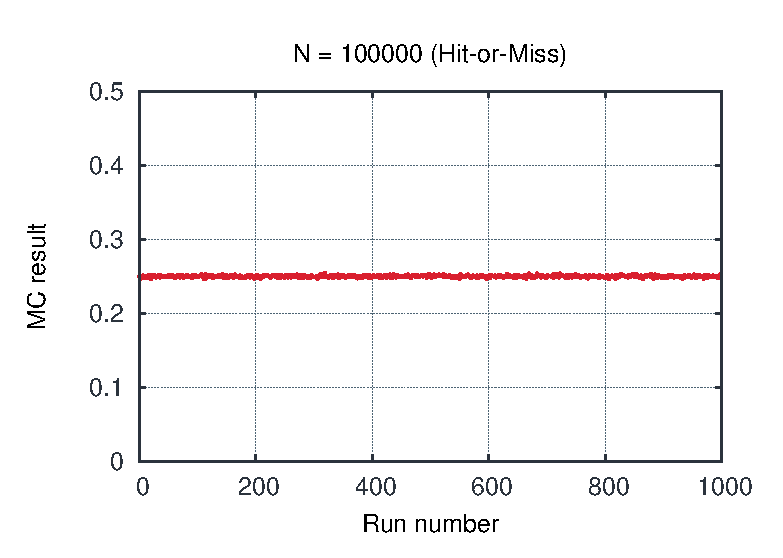
\includegraphics[width=\columnwidth]{figures/int100000.eps}
  }

\vfill\null
\end{emptyslide}


\begin{slide}{Optimization of MC}
\null\vfill

  \twocolumn
  {
    \scalebox{.75}{\usetikzlibrary{calc}

\begin{tikzpicture}

  \draw[>=latex, <->, thick] node[left, yshift = 4cm]{$y$} ++ (0, 4) -- (0, 0) -- node[below, xshift = 2cm]{$x$} ++ (4,0);
  
  \foreach \x in {1,...,200}
  {
    \pgfmathparse{rnd}
    \pgfmathsetmacro{\a}{2.9*\pgfmathresult + 0.05}
    \pgfmathparse{rnd}
    \pgfmathsetmacro{\b}{2.9*\pgfmathresult + 0.05}
    \pgfmathsetmacro{\c}{\a - 2.0 * \b}
        
    \ifthenelse{\lengthtest{\c pt > 0.2 pt}}{\draw[filled, color=pdcolor7] (\a, \b) circle (0.03);}{}
    \ifthenelse{\lengthtest{\c pt < - 0.2 pt}}{\draw[filled, color=pdcolor6] (\a, \b) circle (0.03);}{}
  }

  \draw[ultra thick] (0,0) -- node[yshift = 1.5cm, xshift = 2cm]{$f(x) = \frac{1}{2}x$} ++ (4,2);
  
  \draw[color=pdcolor3, dashed] node[left, yshift = 3cm]{1} ++ (0, 3) -- (3,3) -- node[yshift = -1.75cm]{1} (3, 0);
      
\end{tikzpicture}
}
  }
  {
    \scalebox{.75}{\usetikzlibrary{calc}

\begin{tikzpicture}

  \draw[>=latex, <->, thick] node[left, yshift = 4cm]{$y$} ++ (0, 4) -- (0, 0) -- node[below, xshift = 2cm]{$x$} ++ (4,0);
  
  \foreach \x in {1,...,200}
  {
    \pgfmathparse{rnd}
    \pgfmathsetmacro{\a}{2.9*\pgfmathresult + 0.05}
    \pgfmathparse{rnd}
    \pgfmathsetmacro{\b}{1.4*\pgfmathresult + 0.05}
    \pgfmathsetmacro{\c}{\a - 2.0 * \b}
        
    \ifthenelse{\lengthtest{\c pt > 0.2 pt}}{\draw[filled, color=pdcolor7] (\a, \b) circle (0.03);}{}
    \ifthenelse{\lengthtest{\c pt < - 0.2 pt}}{\draw[filled, color=pdcolor6] (\a, \b) circle (0.03);}{}
  }

  \draw[ultra thick] (0,0) -- node[yshift = 1.5cm, xshift = 2cm]{$f(x) = \frac{1}{2}x$} ++ (4,2);
  
  \draw[color=pdcolor3, dashed] node[left, yshift = 1.5cm]{0.5} ++ (0, 1.5) -- (3,1.5) -- node[yshift = -1.75cm]{1} (3, 0);
      
\end{tikzpicture}
}
  }

  \begin{itemize}
   \item You want to avoid drawing ``red'' points as they do not contribute to your integral
   \item You can choose any rectangle as far as it contains maximum of $f(x)$ in given range
  \end{itemize}

\vfill\null
\end{slide}

\begin{slide}[toc=]{Optimization of MC}
\null\vfill

  \twocolumn
  {
    \begin{itemize}
      \item Lets consider the following function:
  
      $$F(Q^2) = \frac{1}{(1 + Q^2)^2}$$
      {\it\color{pdcolor3} more or less dipole form factor}
      
      \item Integrating this function over $Q^2$ is highly inefficient
      
      \item However, one can integrate by substitution to get better performance, e.g.
      
      $$x = \mbox{log}_{10}(Q^2)$$
      
    \sep{\it\color{pdcolor6}don't forget about Jacobian}

    \end{itemize}

  }
  {
    \usetikzlibrary{calc}

\pgfplotsset{every  tick/.style={pdcolor3,}, minor x tick num=1,}

\begin{tikzpicture}

  \begin{axis}[xlabel = $Q^2$, ylabel = $F(Q^2)$, ylabel near ticks, domain=1:10, scale=0.5, axis lines = left, inner axis line style={>=latex}, ymin = 0, ymax = 0.275, xmin = 1, xmax = 10.5]
    
    \addplot[mark=none, color=pdcolor1, ultra thick] {1 / (1 + x) / (1 + x)};
    \addplot[mark=none, dashed, color=pdcolor3, thick] coordinates {(1,0.25) (10,0.25) (10,0)};

    
    \foreach \x in {1,...,200}
    {
      \pgfmathparse{rnd}
      \pgfmathsetmacro{\a}{9.0*\pgfmathresult + 0.95}
      \pgfmathparse{rnd}
      \pgfmathsetmacro{\b}{0.23*\pgfmathresult + 0.01}
      \pgfmathsetmacro{\c}{\b - 1 / (1 + \a) / (1 + \a)}
      	  
      \ifthenelse{\lengthtest{\c pt > 0.01 pt}}{\addplot[mark=*, mark size = 1pt, color=pdcolor6] coordinates {(\a, \b)};}{}
      \ifthenelse{\lengthtest{\c pt < -0.01 pt}}{\addplot[mark=*, mark size = 1pt, color=pdcolor7] coordinates {(\a, \b)};}{}
    }
    
  \end{axis}

\end{tikzpicture}
    \vspace{-10pt}
    \usetikzlibrary{calc}

\pgfplotsset{every  tick/.style={pdcolor3,}, minor x tick num=1,}

\begin{tikzpicture}

  \begin{axis}[xlabel = {$x = \mbox{log}_{10}(Q^2)$}, ylabel = $F(x)$, ylabel near ticks, domain=-2:1, scale=0.5, axis lines = left, inner axis line style={>=latex}, ymin = 0, ymax = 1.25, xmin = -2, xmax = 1.25]
    
    \addplot[mark=none, color=pdcolor1, ultra thick] {1 / (1 + 10^x) / (1 + 10^x)};
    \addplot[mark=none, dashed, color=pdcolor3, thick] coordinates {(-2,1) (1,1) (1,0)};
    
    \foreach \x in {1,...,200}
    {
      \pgfmathparse{rnd}
      \pgfmathsetmacro{\a}{-2.90*\pgfmathresult + 0.95}
      \pgfmathparse{rnd}
      \pgfmathsetmacro{\b}{0.90*\pgfmathresult + 0.05}
      \pgfmathsetmacro{\d}{-0.175 * (\a + 2) * (\a + 2) + 1}
      \pgfmathsetmacro{\c}{\b - \d}
      	  
      \ifthenelse{\lengthtest{\c pt > 0.1 pt}}{\addplot[mark=*, mark size = 1pt, color=pdcolor6] coordinates {(\a, \b)};}{}
      \ifthenelse{\lengthtest{\c pt < - 0.1 pt}}{\addplot[mark=*, mark size = 1pt, color=pdcolor7] coordinates {(\a, \b)};}{}
    }
    
  \end{axis}

\end{tikzpicture}
    
  }
    
\vfill\null
\end{slide}

\begin{slide}[toc=Crude method]{MC integration (Crude method)}
\null\vfill

  Lets do the following integration using MC method once again:
  
  $$\int_0^1 f(x)dx = \int_0^1 \left(\frac{1}{2}x\right) dx = \left.\frac{1}{2}\frac{x^2}{2}\right|_{0}^{1} = \frac{1}{4}$$
  \twocolumn
  {
    \begin{itemize}
      \item One can approximate integral
      \vspace{-5pt}
      $$\int_a^b f(x) dx \approx \frac{b - a}{N}\sum_{i=1}^{N} f(x_i)$$
     
      where $x_i$ is a random number from $[a, b]$
      
      \item It can be shown that Crude method is more accurate than Hit-or-Miss
      
      \item We will skip the math and look at some comparisons
      
    \end{itemize}
  }
  {
    \usetikzlibrary{calc}

\begin{tikzpicture}

  \draw[>=latex, <->, thick] node[left, yshift = 4cm]{$y$} ++ (0, 4) -- (0, 0) -- node[below, xshift = 2cm]{$x$} ++ (4,0);
  
  \foreach \x in {1,...,14}
  {
    \pgfmathparse{rnd}

    \pgfmathsetmacro{\a}{0.2 * \x + 0.05 + 0.1 * \pgfmathresult - 0.05}
        
    \draw[filled, color=pdcolor7] (\a, 0) circle (0.03);
    
    \draw[thin, color=pdcolor3, dashed] (\a, 0) -- (\a, 0.5*\a);
  }

  \draw[ultra thick] (0,0) -- node[yshift = 1.5cm, xshift = 2cm]{$f(x) = \frac{1}{2}x$} ++ (4,2);
        
\end{tikzpicture}

  }

\vfill\null
\end{slide}

\begin{emptyslide}{Methods comparison}
\null\vfill

  \twocolumn
  {
    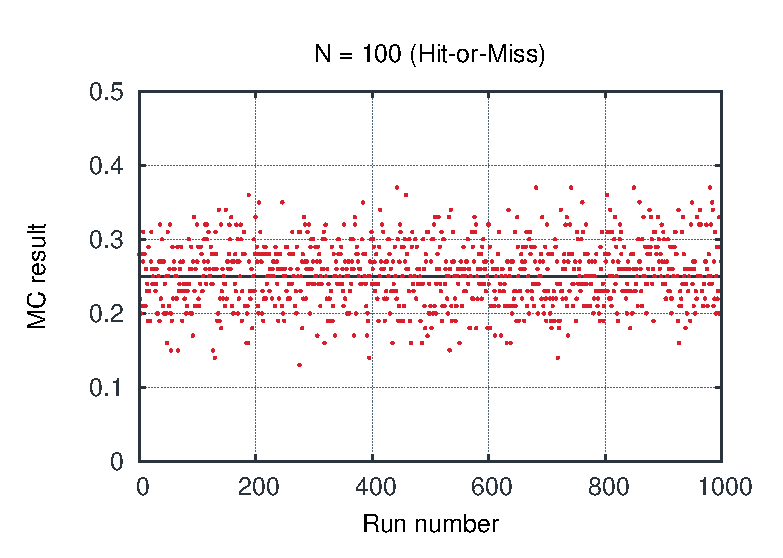
\includegraphics[width=\columnwidth]{figures/int100.eps}
    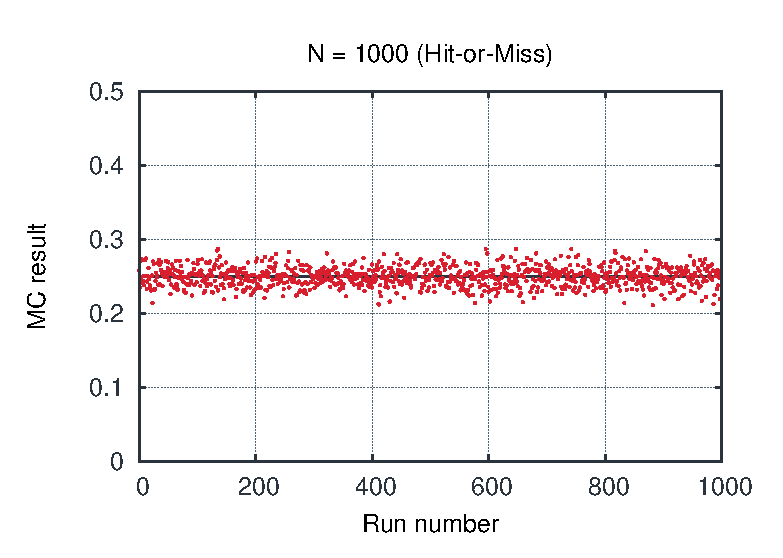
\includegraphics[width=\columnwidth]{figures/int1000.eps}
  }
  {
    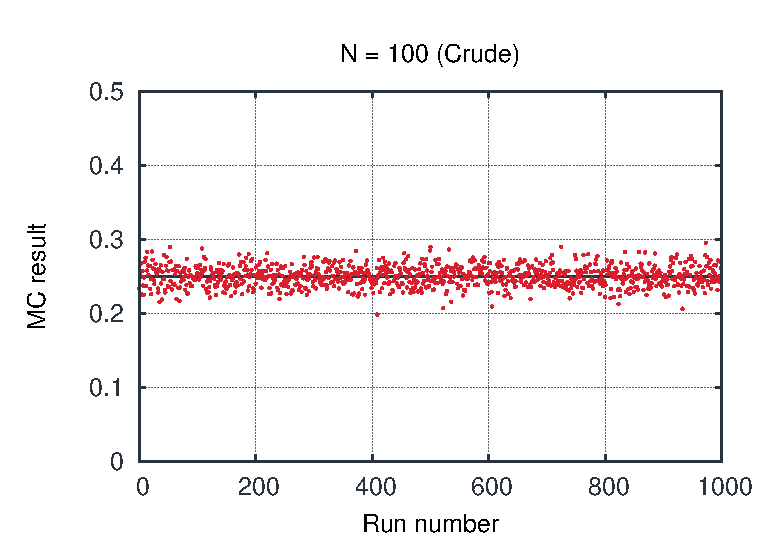
\includegraphics[width=\columnwidth]{figures/int2100.eps}
    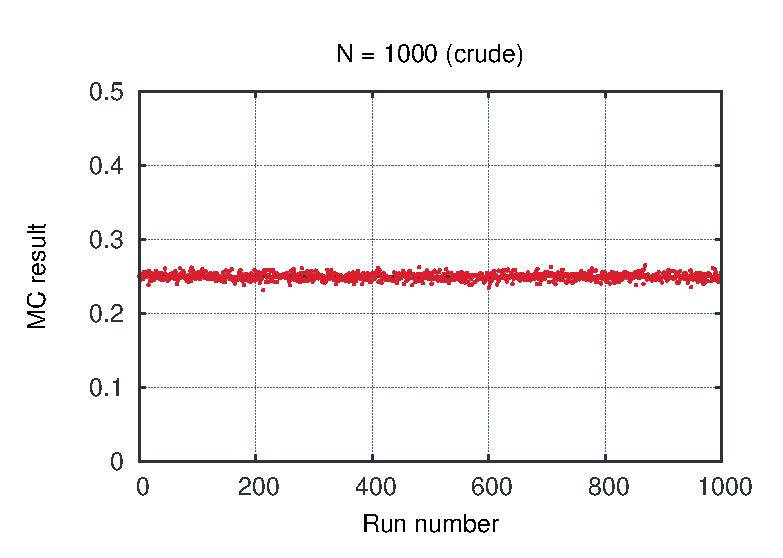
\includegraphics[width=\columnwidth]{figures/int21000.eps}
  }

\vfill\null
\end{emptyslide}

